\section{Variable Bias Voltage SRF T$_B$ Residuals}
%==================================================
\label{app:Vset_dtb_data_plots}

\subsection{Channel 1}
\begin{figure}[H]
  \label{fig:Vset.ch1_dtb}
  \centering
  \hspace{1.5cm}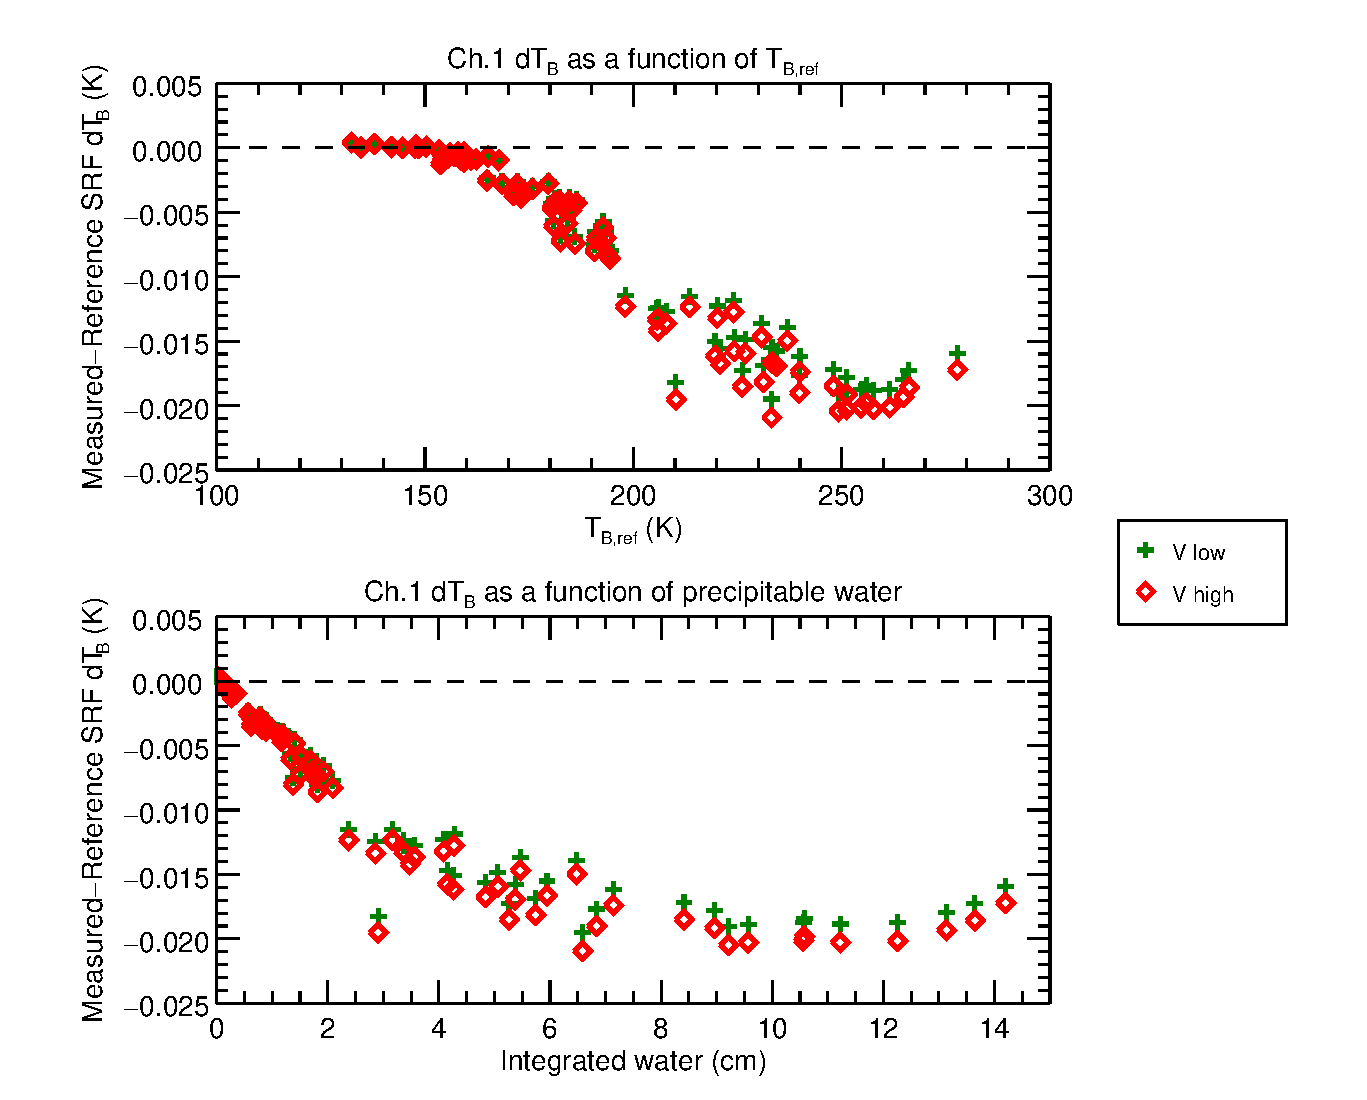
\includegraphics[scale=0.45]{graphics/dtb/Vset/atms_npp.ch1.dTb_T_PW_stats.eps}
  \caption{ATMS channel 1 differences in brightness temperatures as a function of $T_B$ (top) and total preciptable water (bottom) for $V_{LO}$ and $V_{HI}$ compared to nominal bias voltage at nominal temperature (20\textdegree{}C). MonoRTM v5.0 was used with $\epsilon=0.6$ and $r=0.4$ for the ECMWF83 profile set.}
\end{figure}

\subsection{Channel 2}
\begin{figure}[H]
  \label{fig:Vset.ch2_dtb}
  \centering
  \hspace{1.5cm}\includegraphics[scale=0.45]{graphics/dtb/Vset/atms_npp.ch2.dTb_T_PW_stats.eps}
  \caption{ATMS channel 2 differences in brightness temperatures as a function of $T_B$ (top) and total preciptable water (bottom) for $V_{LO}$ and $V_{HI}$ compared to nominal bias voltage at nominal temperature (20\textdegree{}C). MonoRTM v5.0 was used with $\epsilon=0.6$ and $r=0.4$ for the ECMWF83 profile set.}
\end{figure}

\subsection{Channel 3}
\begin{figure}[H]
  \label{fig:Vset.ch3_dtb}
  \centering
  \hspace{1.5cm}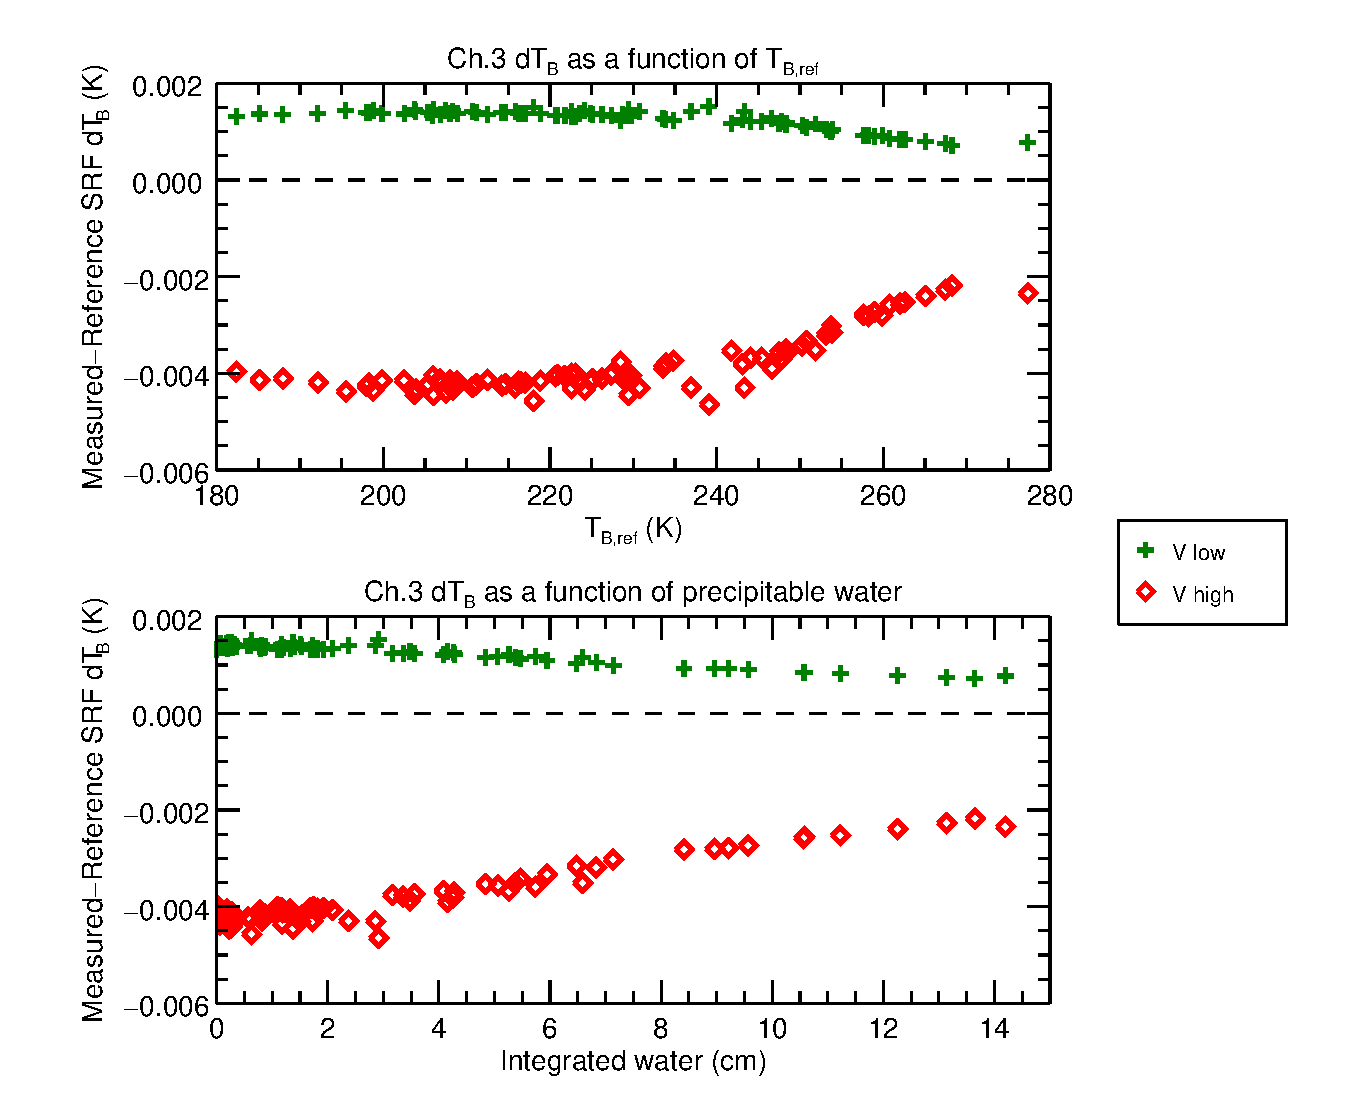
\includegraphics[scale=0.45]{graphics/dtb/Vset/atms_npp.ch3.dTb_T_PW_stats.eps}
  \caption{ATMS channel 3 differences in brightness temperatures as a function of $T_B$ (top) and total preciptable water (bottom) for $V_{LO}$ and $V_{HI}$ compared to nominal bias voltage at nominal temperature (20\textdegree{}C). MonoRTM v5.0 was used with $\epsilon=0.6$ and $r=0.4$ for the ECMWF83 profile set.}
\end{figure}

\subsection{Channel 4}
\begin{figure}[H]
  \label{fig:Vset.ch4_dtb}
  \centering
  \hspace{1.5cm}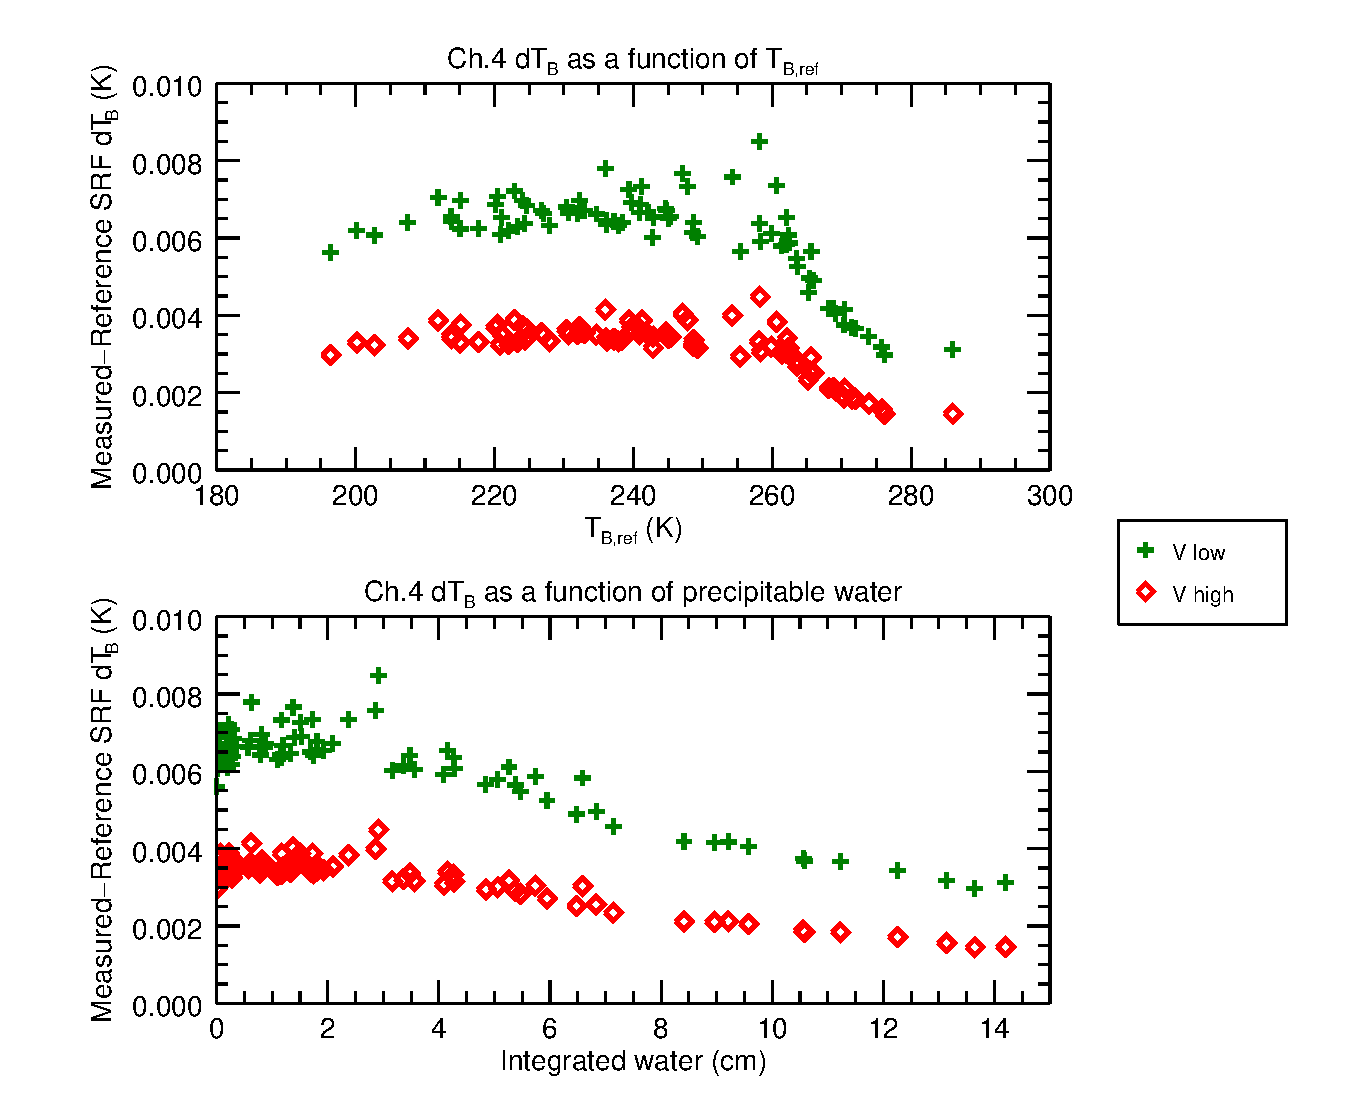
\includegraphics[scale=0.45]{graphics/dtb/Vset/atms_npp.ch4.dTb_T_PW_stats.eps}
  \caption{ATMS channel 4 differences in brightness temperatures as a function of $T_B$ (top) and total preciptable water (bottom) for $V_{LO}$ and $V_{HI}$ compared to nominal bias voltage at nominal temperature (20\textdegree{}C). MonoRTM v5.0 was used with $\epsilon=0.6$ and $r=0.4$ for the ECMWF83 profile set.}
\end{figure}

\subsection{Channel 5}
\begin{figure}[H]
  \label{fig:Vset.ch5_dtb}
  \centering
  \hspace{1.5cm}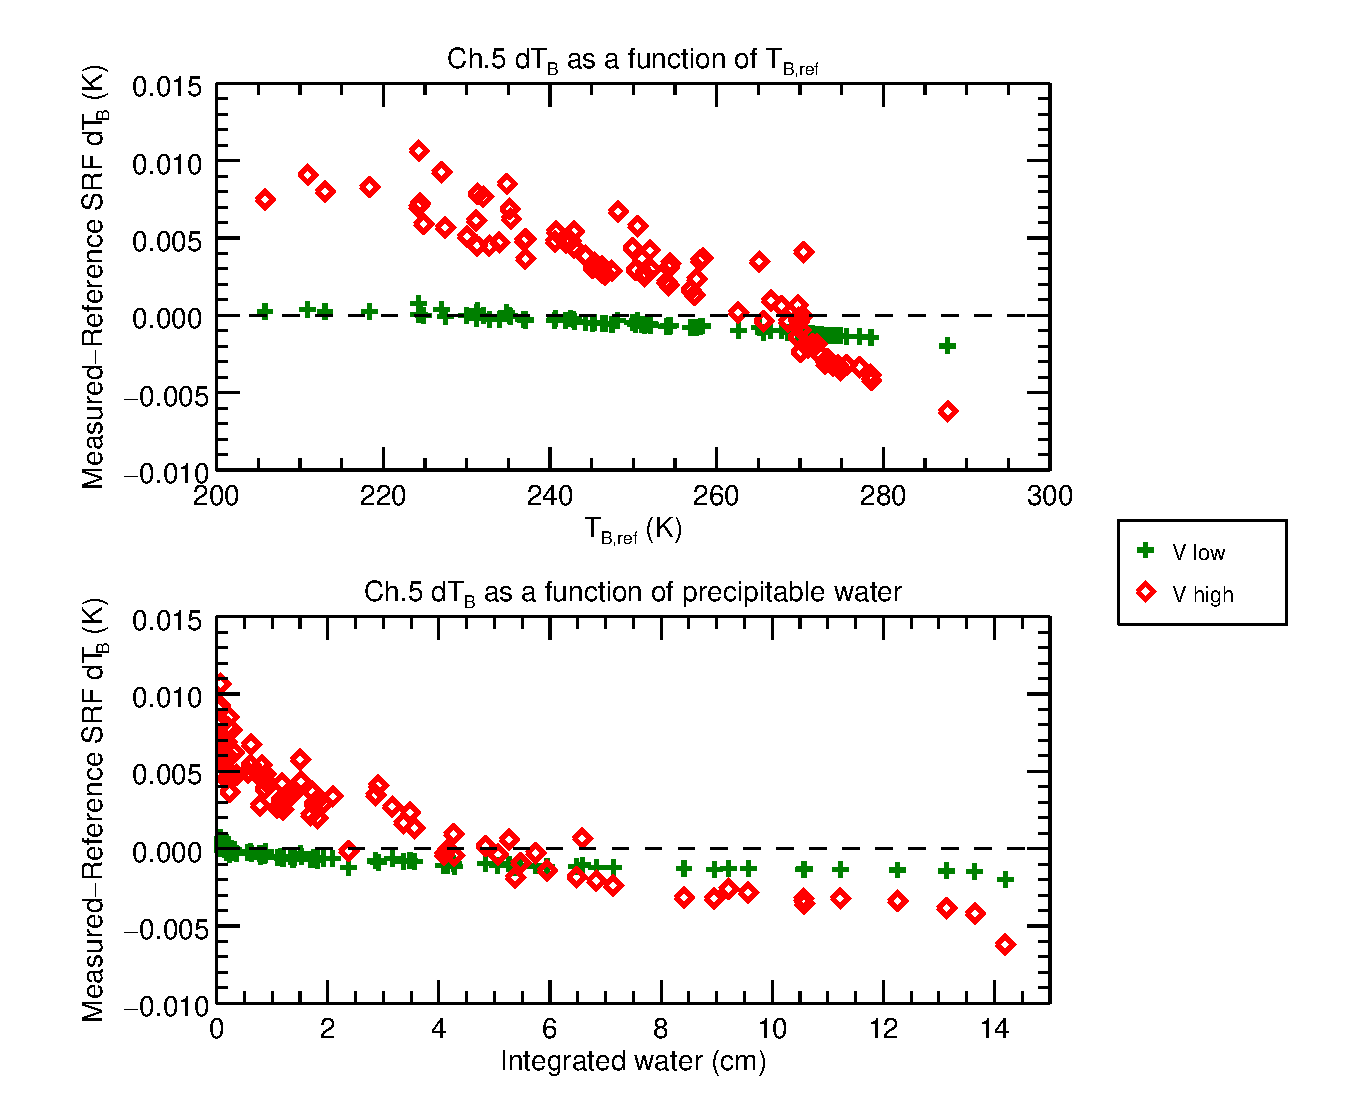
\includegraphics[scale=0.45]{graphics/dtb/Vset/atms_npp.ch5.dTb_T_PW_stats.eps}
  \caption{ATMS channel 5 differences in brightness temperatures as a function of $T_B$ (top) and total preciptable water (bottom) for $V_{LO}$ and $V_{HI}$ compared to nominal bias voltage at nominal temperature (20\textdegree{}C). MonoRTM v5.0 was used with $\epsilon=0.6$ and $r=0.4$ for the ECMWF83 profile set.}
\end{figure}

\subsection{Channel 6}
\begin{figure}[H]
  \label{fig:Vset.ch6_dtb}
  \centering
  \hspace{1.5cm}\includegraphics[scale=0.45]{graphics/dtb/Vset/atms_npp.ch6.dTb_T_PW_stats.eps}
  \caption{ATMS channel 6 differences in brightness temperatures as a function of $T_B$ (top) and total preciptable water (bottom) for $V_{LO}$ and $V_{HI}$ compared to nominal bias voltage at nominal temperature (20\textdegree{}C). MonoRTM v5.0 was used with $\epsilon=0.6$ and $r=0.4$ for the ECMWF83 profile set.}
\end{figure}

\subsection{Channel 7}
\begin{figure}[H]
  \label{fig:Vset.ch7_dtb}
  \centering
  \hspace{1.5cm}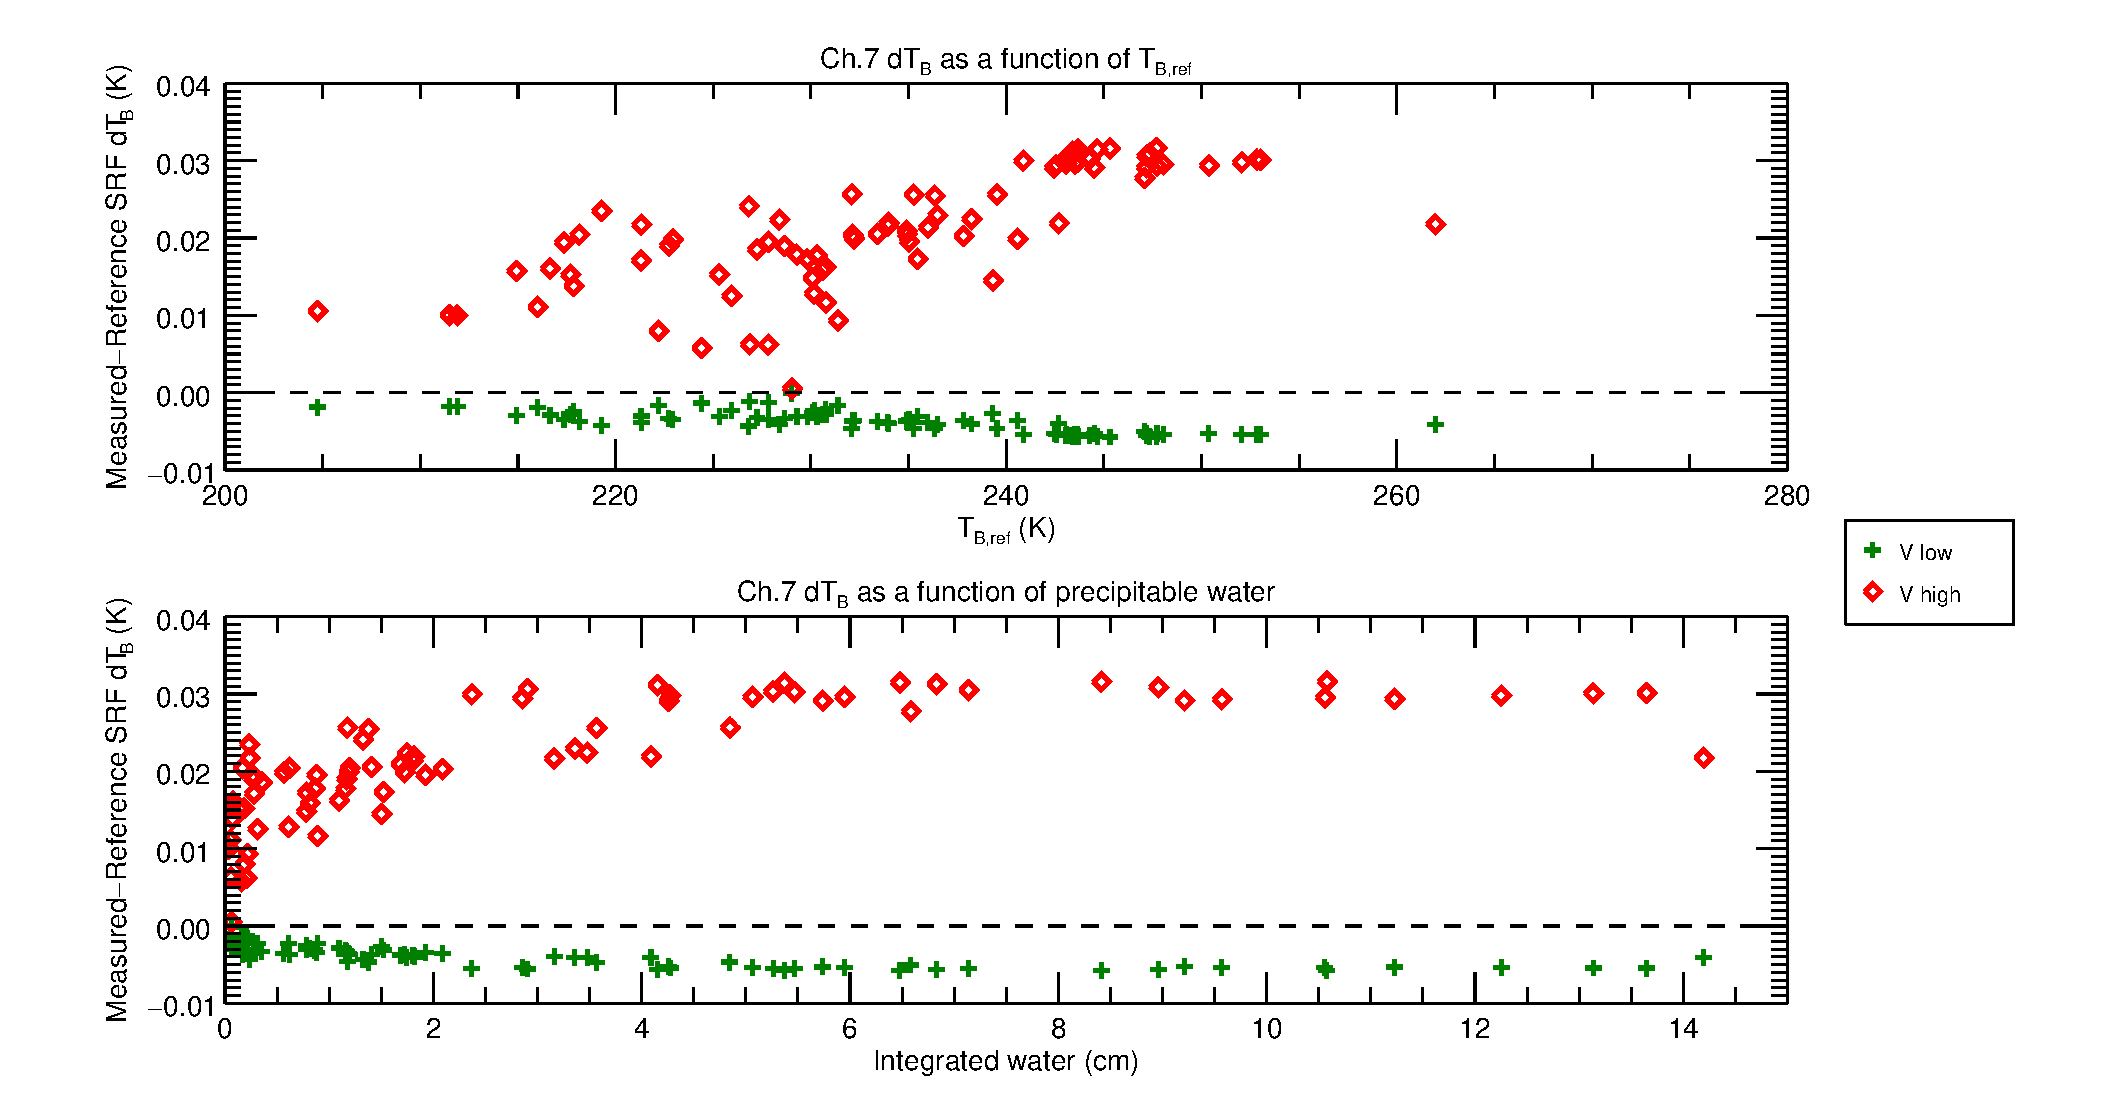
\includegraphics[scale=0.45]{graphics/dtb/Vset/atms_npp.ch7.dTb_T_PW_stats.eps}
  \caption{ATMS channel 7 differences in brightness temperatures as a function of $T_B$ (top) and total preciptable water (bottom) for $V_{LO}$ and $V_{HI}$ compared to nominal bias voltage at nominal temperature (20\textdegree{}C). MonoRTM v5.0 was used with $\epsilon=0.6$ and $r=0.4$ for the ECMWF83 profile set.}
\end{figure}

\subsection{Channel 8}
\begin{figure}[H]
  \label{fig:Vset.ch8_dtb}
  \centering
  \hspace{1.5cm}\includegraphics[scale=0.45]{graphics/dtb/Vset/atms_npp.ch8.dTb_T_PW_stats.eps}
  \caption{ATMS channel 8 differences in brightness temperatures as a function of $T_B$ (top) and total preciptable water (bottom) for $V_{LO}$ and $V_{HI}$ compared to nominal bias voltage at nominal temperature (20\textdegree{}C). MonoRTM v5.0 was used with $\epsilon=0.6$ and $r=0.4$ for the ECMWF83 profile set.}
\end{figure}

\subsection{Channel 9}
\begin{figure}[H]
  \label{fig:Vset.ch9_dtb}
  \centering
  \hspace{1.5cm}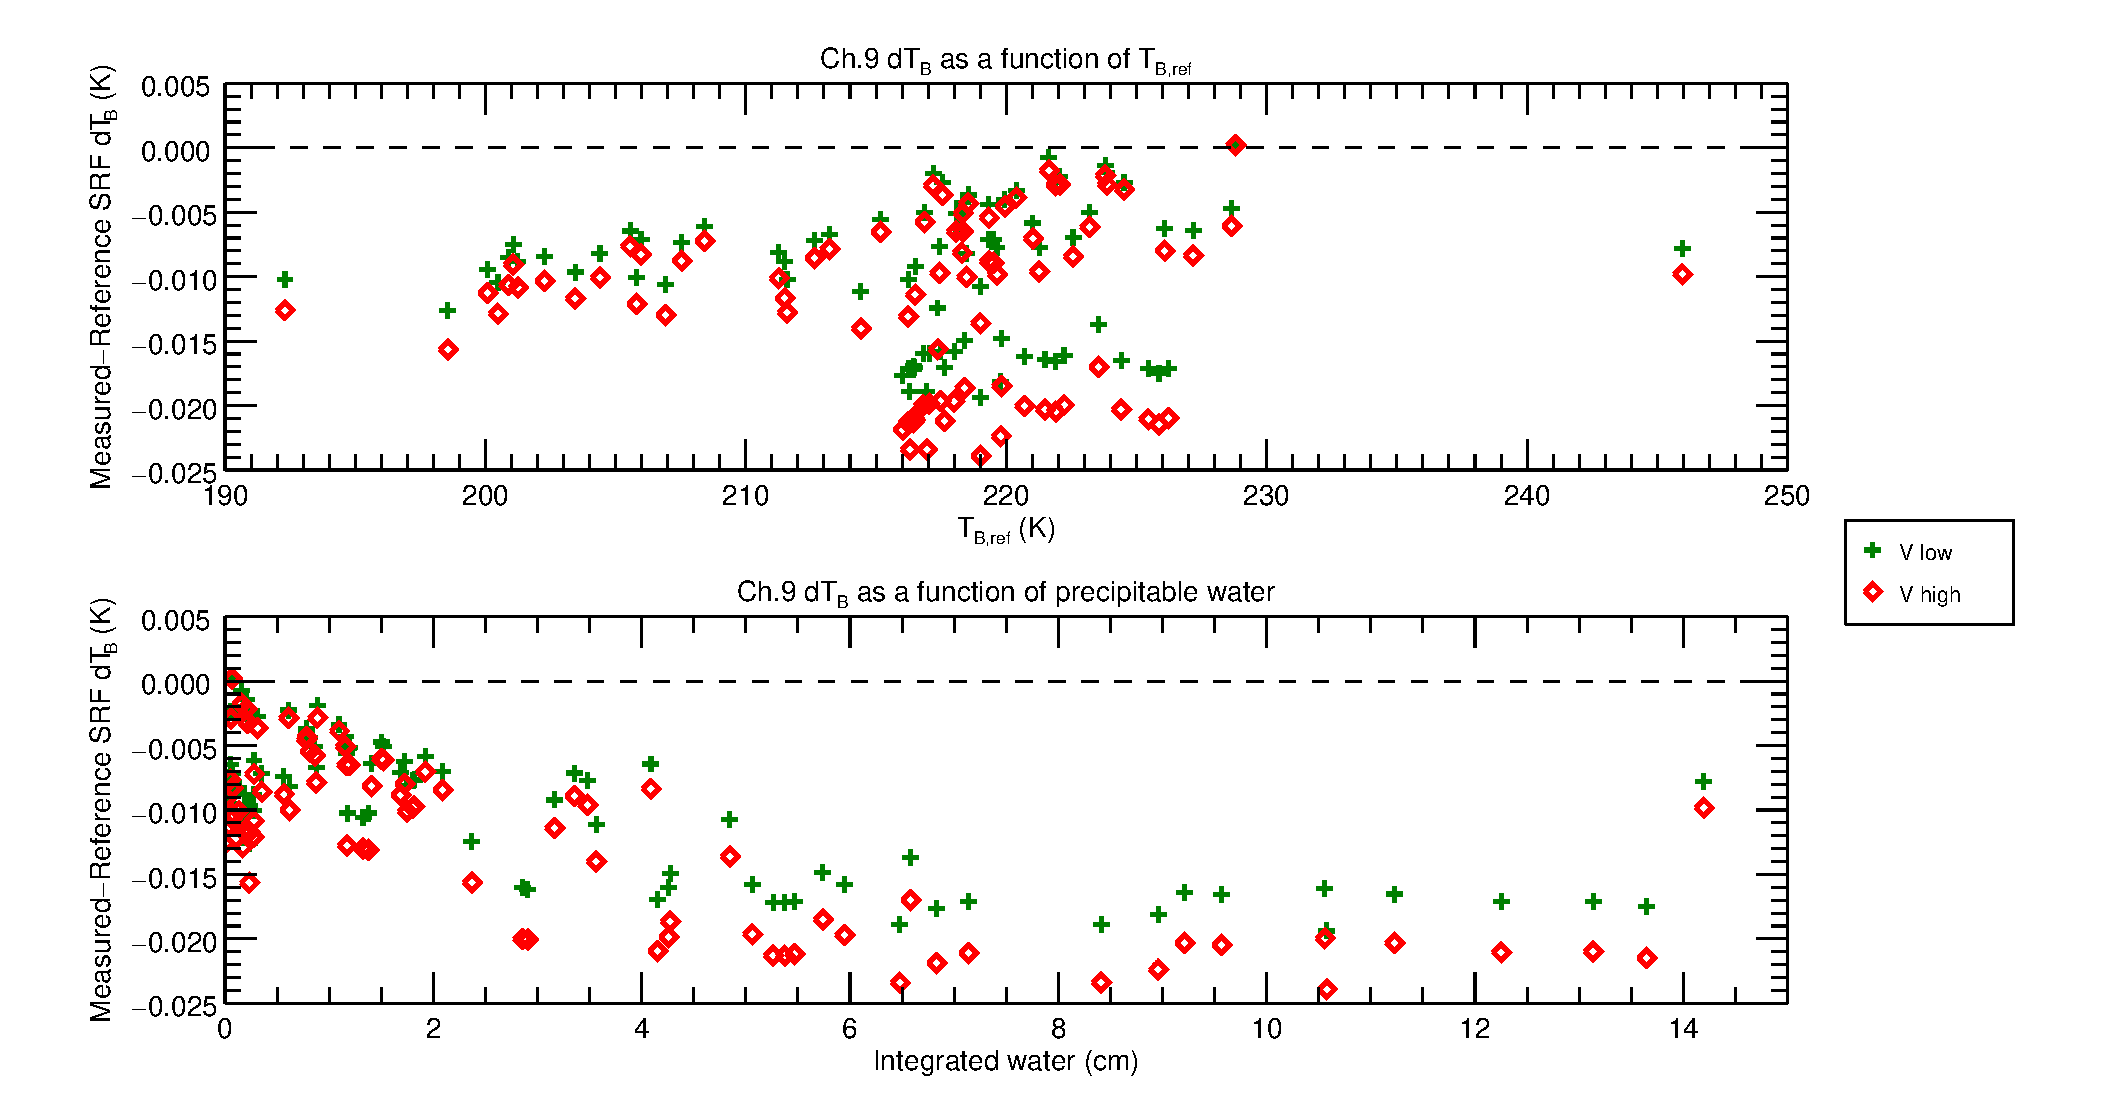
\includegraphics[scale=0.45]{graphics/dtb/Vset/atms_npp.ch9.dTb_T_PW_stats.eps}
  \caption{ATMS channel 9 differences in brightness temperatures as a function of $T_B$ (top) and total preciptable water (bottom) for $V_{LO}$ and $V_{HI}$ compared to nominal bias voltage at nominal temperature (20\textdegree{}C). MonoRTM v5.0 was used with $\epsilon=0.6$ and $r=0.4$ for the ECMWF83 profile set.}
\end{figure}

\subsection{Channel 10}
\begin{figure}[H]
  \label{fig:Vset.ch10_dtb}
  \centering
  \hspace{1.5cm}\includegraphics[scale=0.45]{graphics/dtb/Vset/atms_npp.ch10.dTb_T_PW_stats.eps}
  \caption{ATMS channel 10 differences in brightness temperatures as a function of $T_B$ (top) and total preciptable water (bottom) for $V_{LO}$ and $V_{HI}$ compared to nominal bias voltage at nominal temperature (20\textdegree{}C). MonoRTM v5.0 was used with $\epsilon=0.6$ and $r=0.4$ for the ECMWF83 profile set.}
\end{figure}

\subsection{Channel 11}
\begin{figure}[H]
  \label{fig:Vset.ch11_dtb}
  \centering
  \hspace{1.5cm}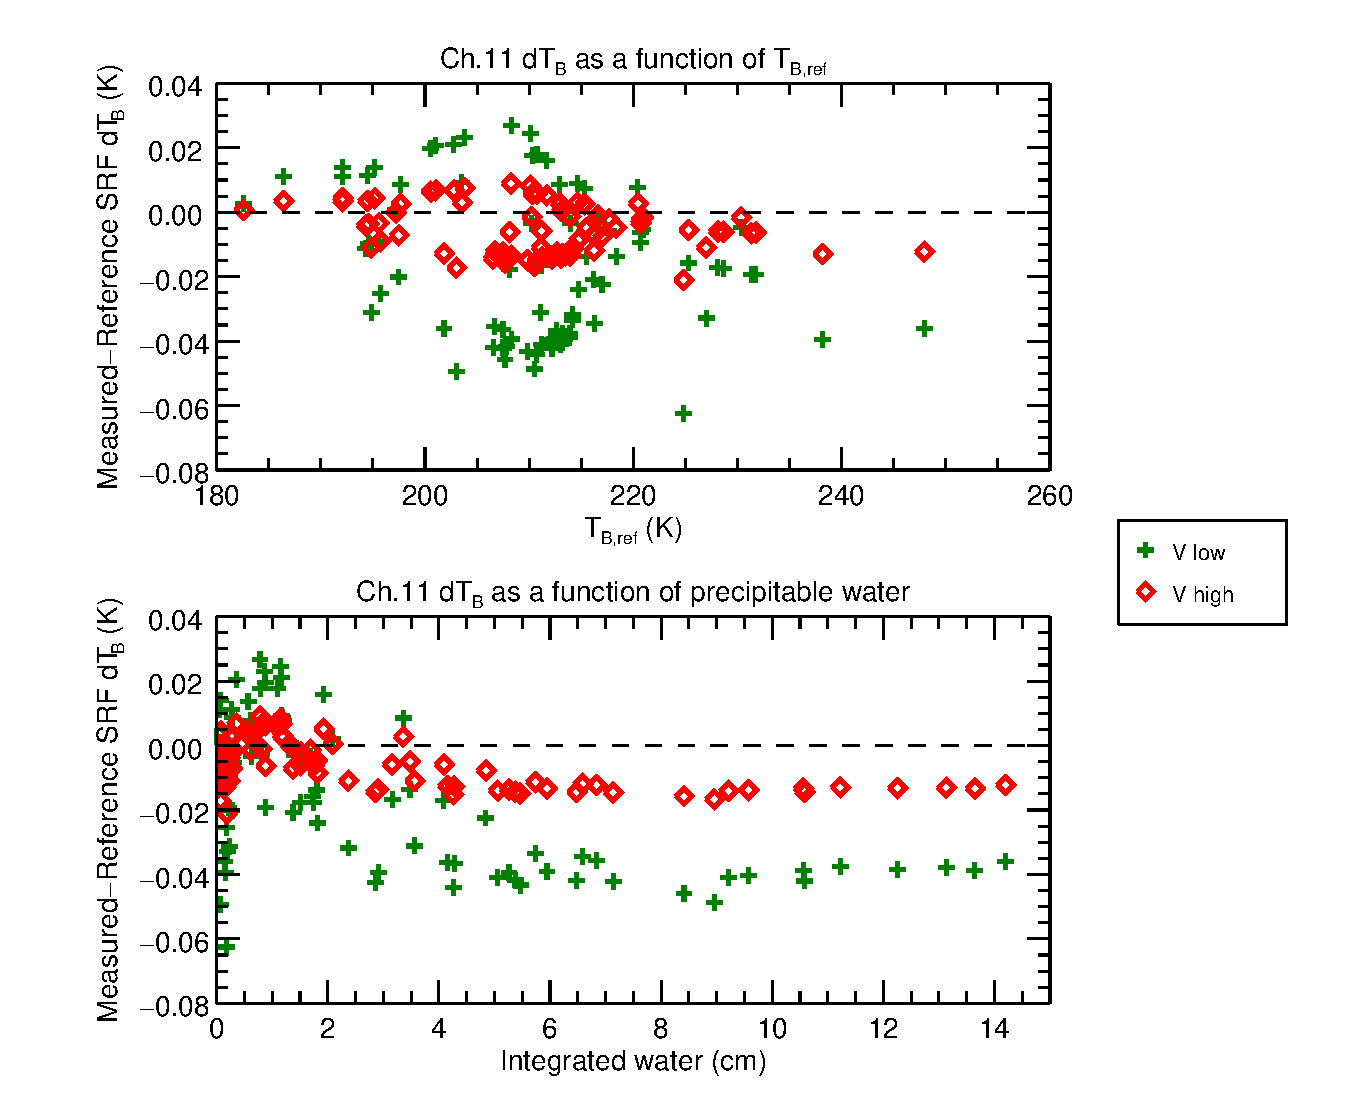
\includegraphics[scale=0.45]{graphics/dtb/Vset/atms_npp.ch11.dTb_T_PW_stats.eps}
  \caption{ATMS channel 11 differences in brightness temperatures as a function of $T_B$ (top) and total preciptable water (bottom) for $V_{LO}$ and $V_{HI}$ compared to nominal bias voltage at nominal temperature (20\textdegree{}C). MonoRTM v5.0 was used with $\epsilon=0.6$ and $r=0.4$ for the ECMWF83 profile set.}
\end{figure}

\subsection{Channel 12}
\begin{figure}[H]
  \label{fig:Vset.ch12_dtb}
  \centering
  \hspace{1.5cm}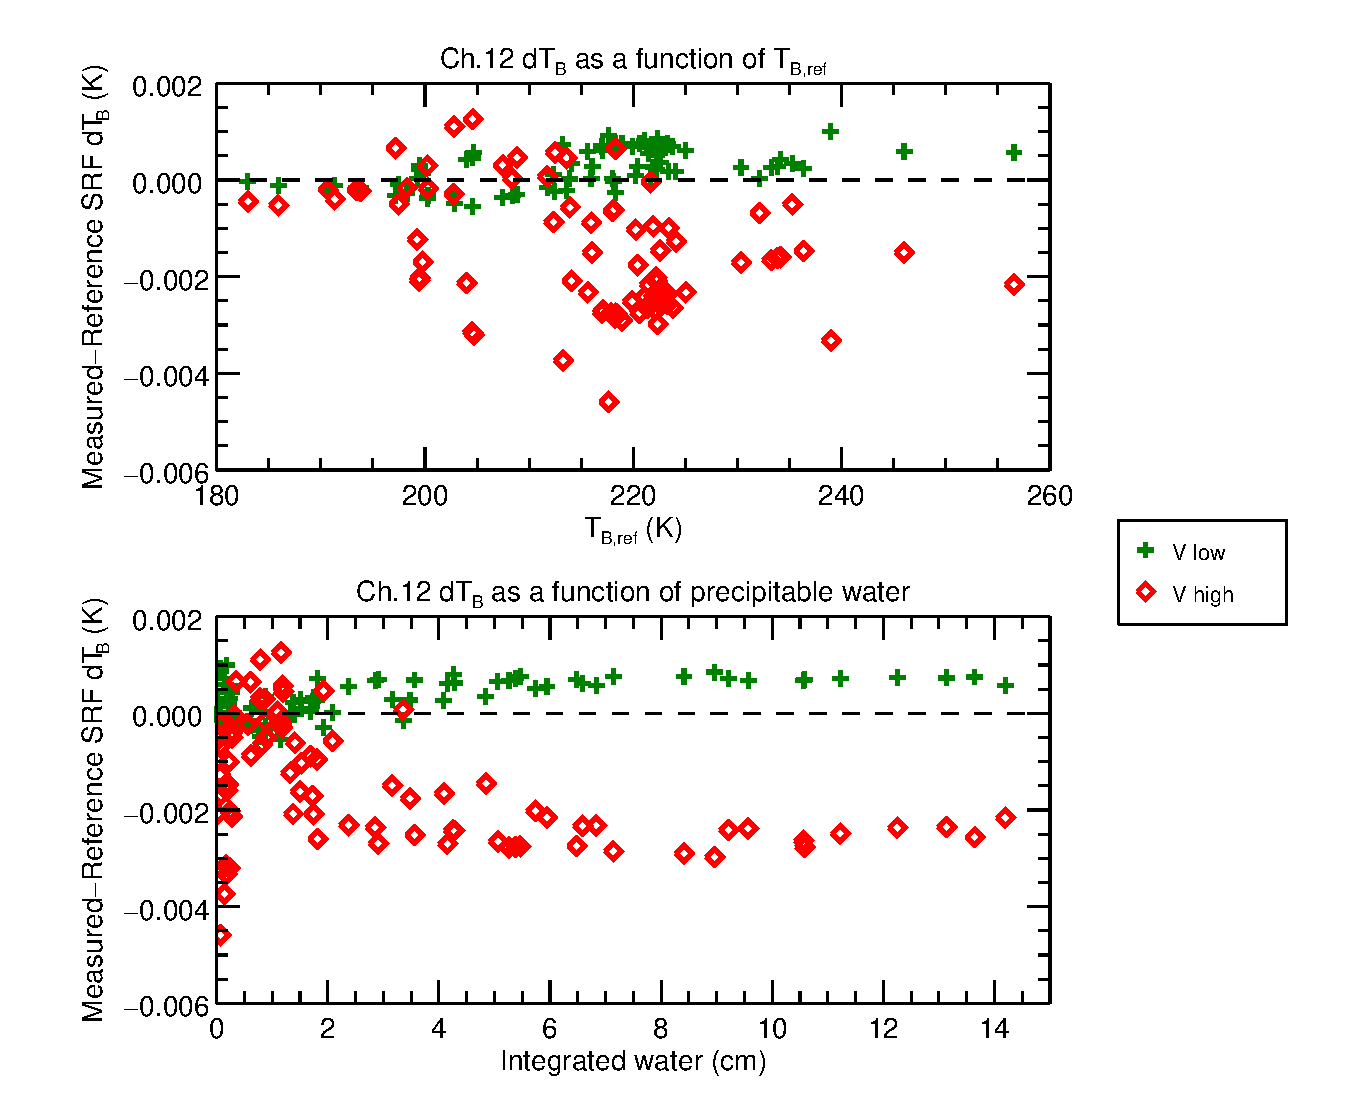
\includegraphics[scale=0.45]{graphics/dtb/Vset/atms_npp.ch12.dTb_T_PW_stats.eps}
  \caption{ATMS channel 12 differences in brightness temperatures as a function of $T_B$ (top) and total preciptable water (bottom) for $V_{LO}$ and $V_{HI}$ compared to nominal bias voltage at nominal temperature (20\textdegree{}C). MonoRTM v5.0 was used with $\epsilon=0.6$ and $r=0.4$ for the ECMWF83 profile set.}
\end{figure}

\subsection{Channel 13}
\begin{figure}[H]
  \label{fig:Vset.ch13_dtb}
  \centering
  \hspace{1.5cm}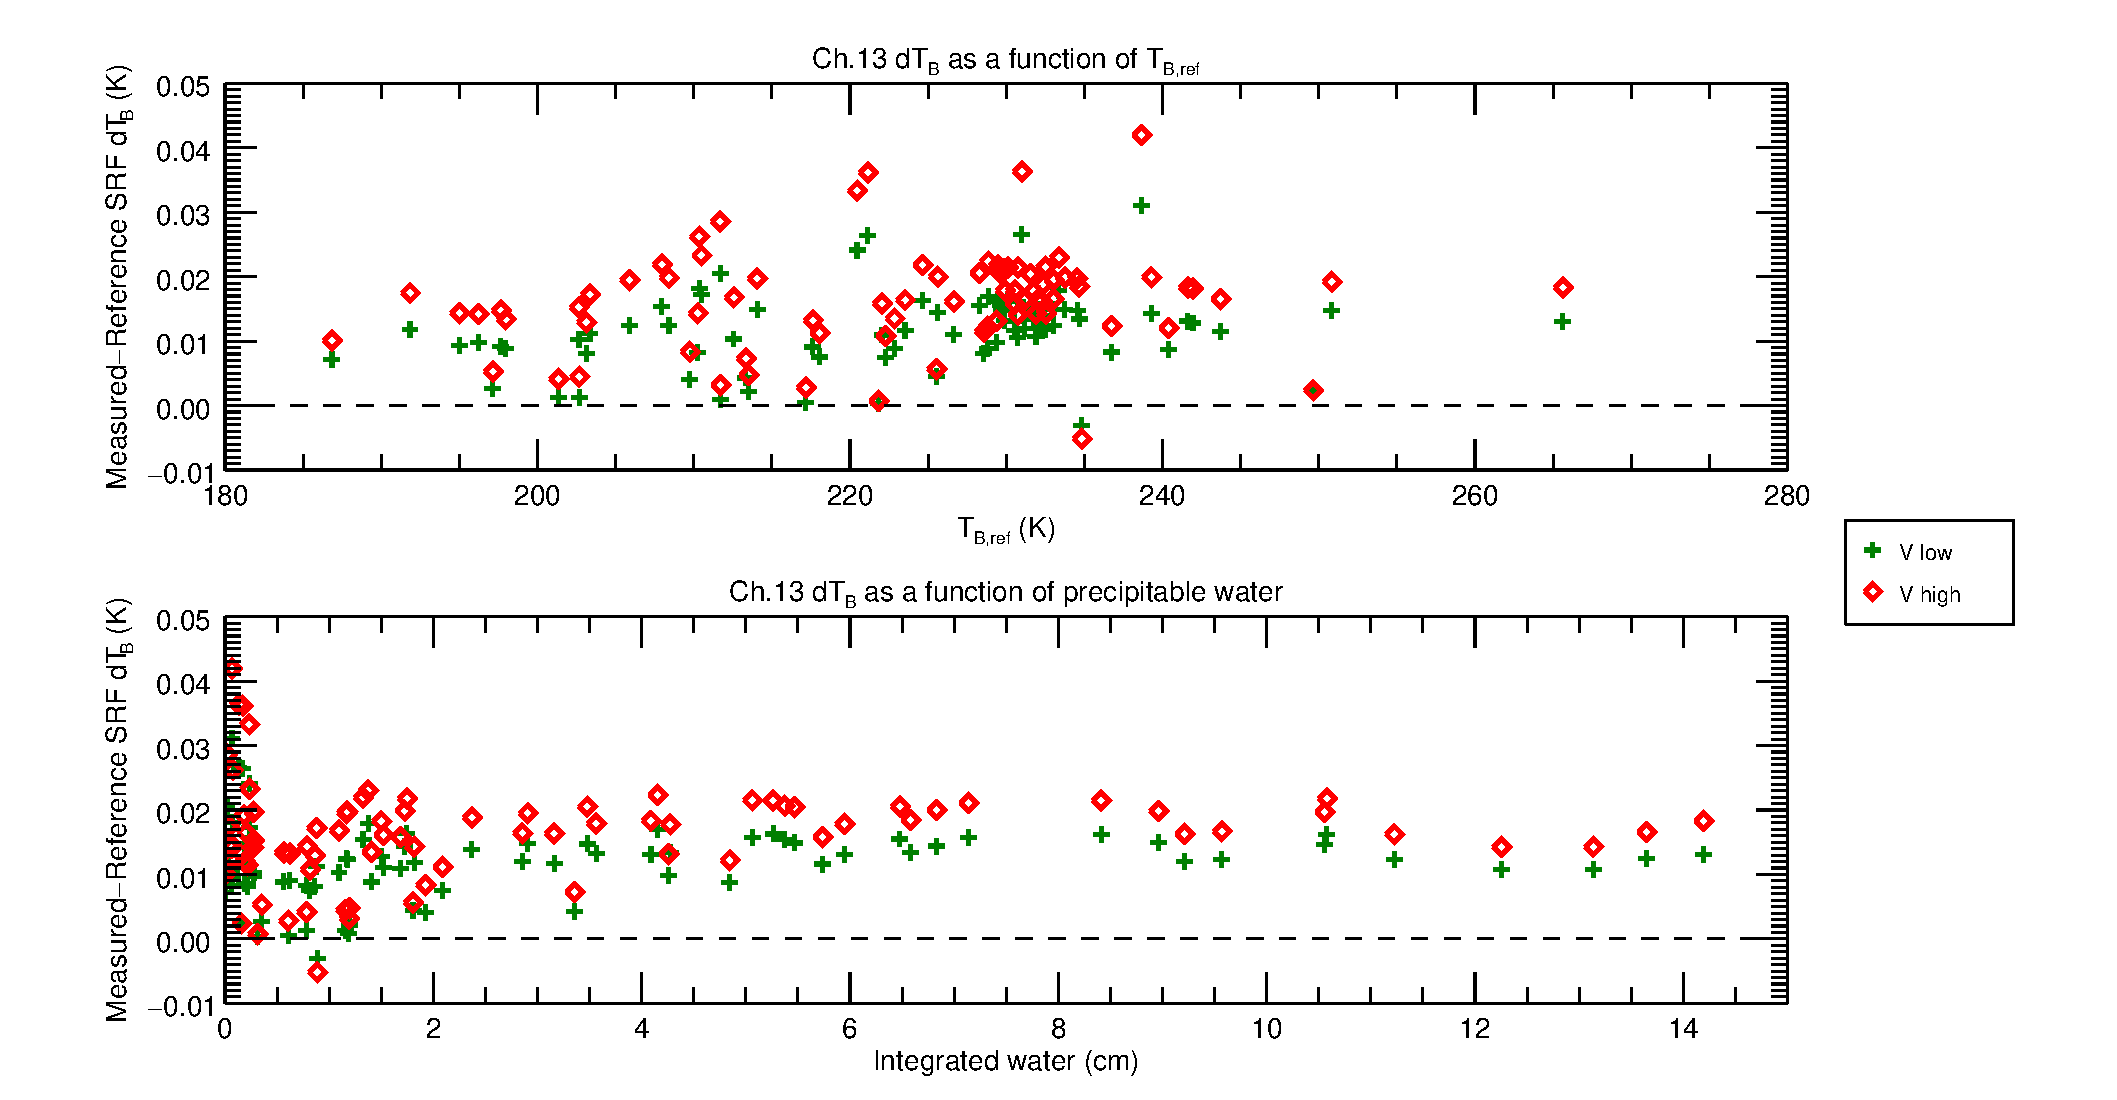
\includegraphics[scale=0.45]{graphics/dtb/Vset/atms_npp.ch13.dTb_T_PW_stats.eps}
  \caption{ATMS channel 13 differences in brightness temperatures as a function of $T_B$ (top) and total preciptable water (bottom) for $V_{LO}$ and $V_{HI}$ compared to nominal bias voltage at nominal temperature (20\textdegree{}C). MonoRTM v5.0 was used with $\epsilon=0.6$ and $r=0.4$ for the ECMWF83 profile set.}
\end{figure}

\subsection{Channel 14}
\begin{figure}[H]
  \label{fig:Vset.ch14_dtb}
  \centering
  \hspace{1.5cm}\includegraphics[scale=0.45]{graphics/dtb/Vset/atms_npp.ch14.dTb_T_PW_stats.eps}
  \caption{ATMS channel 14 differences in brightness temperatures as a function of $T_B$ (top) and total preciptable water (bottom) for $V_{LO}$ and $V_{HI}$ compared to nominal bias voltage at nominal temperature (20\textdegree{}C). MonoRTM v5.0 was used with $\epsilon=0.6$ and $r=0.4$ for the ECMWF83 profile set.}
\end{figure}

\subsection{Channel 15}
\begin{figure}[H]
  \label{fig:Vset.ch15_dtb}
  \centering
  \hspace{1.5cm}\includegraphics[scale=0.45]{graphics/dtb/Vset/atms_npp.ch15.dTb_T_PW_stats.eps}
  \caption{ATMS channel 15 differences in brightness temperatures as a function of $T_B$ (top) and total preciptable water (bottom) for $V_{LO}$ and $V_{HI}$ compared to nominal bias voltage at nominal temperature (20\textdegree{}C). MonoRTM v5.0 was used with $\epsilon=0.6$ and $r=0.4$ for the ECMWF83 profile set.}
\end{figure}

\subsection{Channel 16}
\begin{figure}[H]
  \label{fig:Vset.ch16_dtb}
  \centering
  \hspace{1.5cm}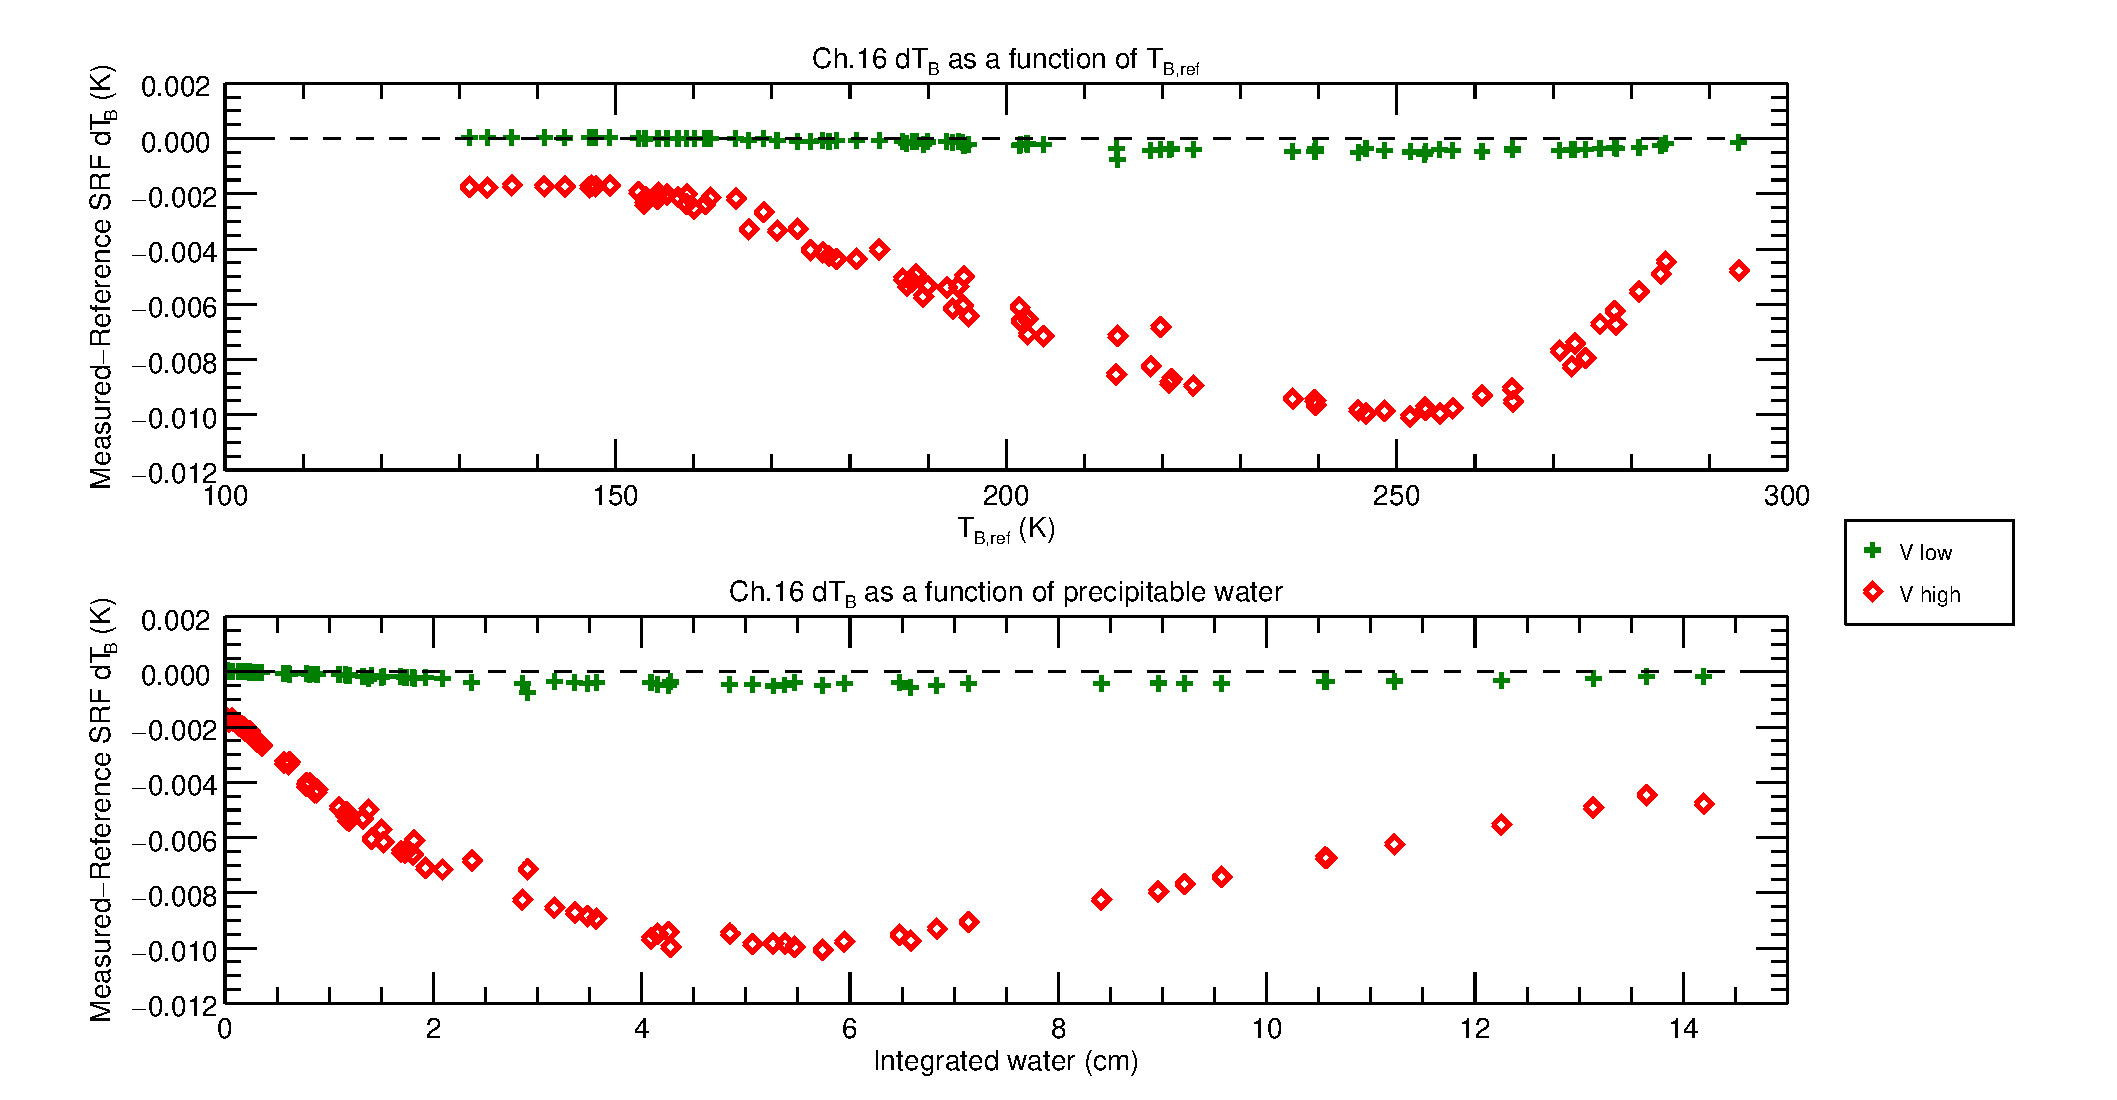
\includegraphics[scale=0.45]{graphics/dtb/Vset/atms_npp.ch16.dTb_T_PW_stats.eps}
  \caption{ATMS channel 16 differences in brightness temperatures as a function of $T_B$ (top) and total preciptable water (bottom) for $V_{LO}$ and $V_{HI}$ compared to nominal bias voltage at nominal temperature (20\textdegree{}C). MonoRTM v5.0 was used with $\epsilon=0.6$ and $r=0.4$ for the ECMWF83 profile set.}
\end{figure}

\subsection{Channel 17}
\begin{figure}[H]
  \label{fig:Vset.ch17_dtb}
  \centering
  \hspace{1.5cm}\includegraphics[scale=0.45]{graphics/dtb/Vset/atms_npp.ch17.dTb_T_PW_stats.eps}
  \caption{ATMS channel 17 differences in brightness temperatures as a function of $T_B$ (top) and total preciptable water (bottom) for $V_{LO}$ and $V_{HI}$ compared to nominal bias voltage at nominal temperature (20\textdegree{}C). MonoRTM v5.0 was used with $\epsilon=0.6$ and $r=0.4$ for the ECMWF83 profile set.}
\end{figure}

\subsection{Channel 18}
\begin{figure}[H]
  \label{fig:Vset.ch18_dtb}
  \centering
  \hspace{1.5cm}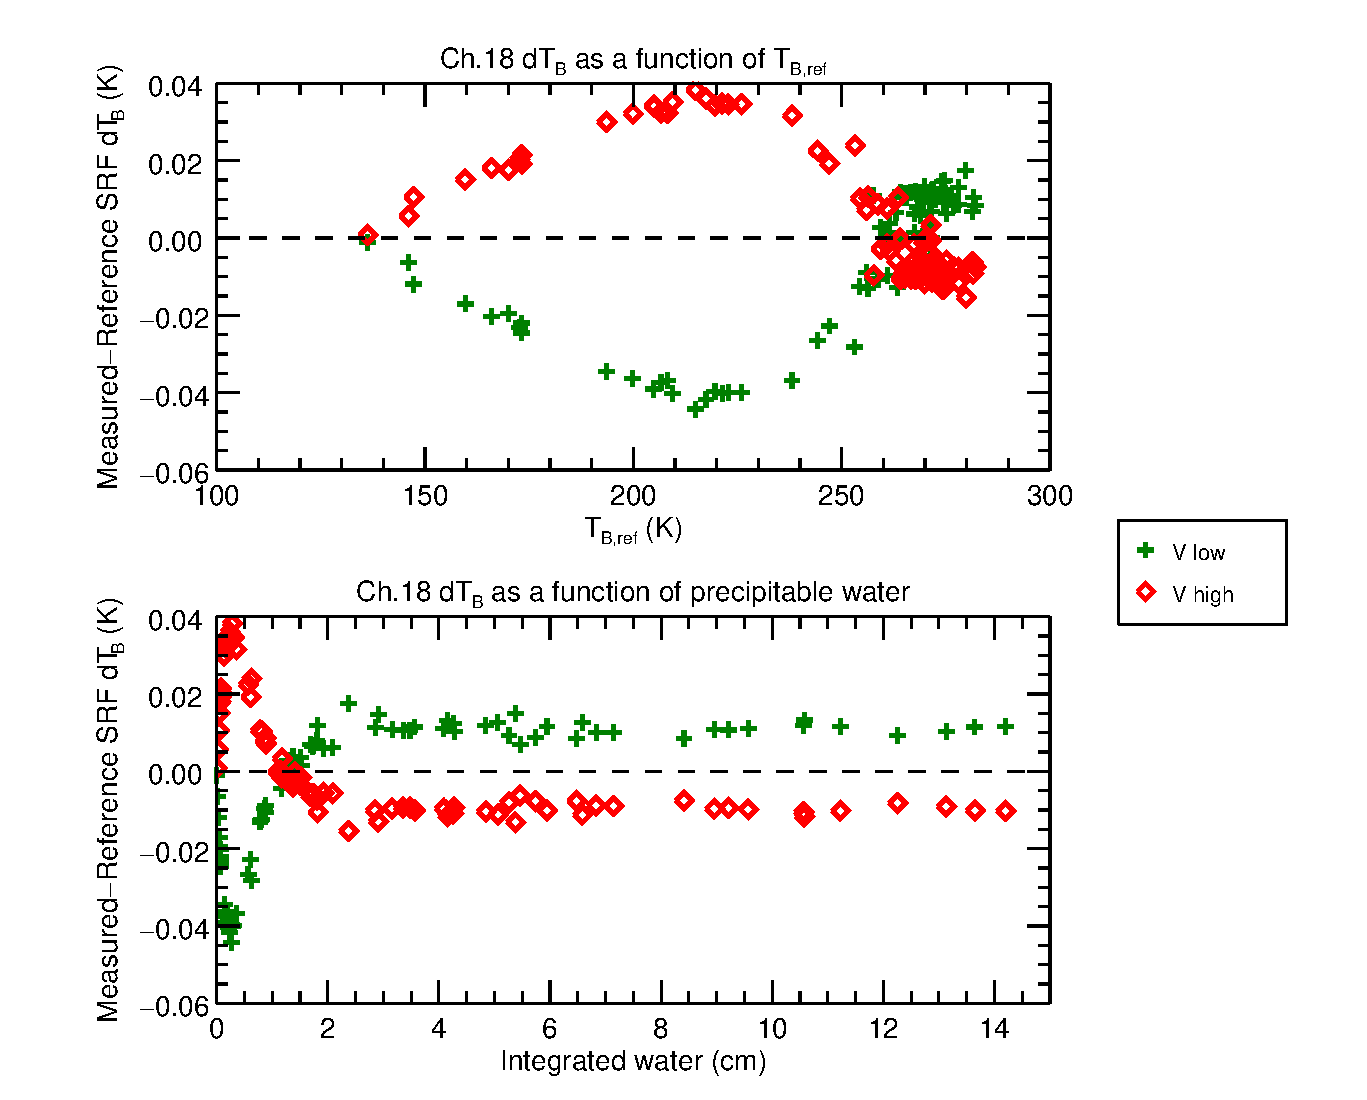
\includegraphics[scale=0.45]{graphics/dtb/Vset/atms_npp.ch18.dTb_T_PW_stats.eps}
  \caption{ATMS channel 18 differences in brightness temperatures as a function of $T_B$ (top) and total preciptable water (bottom) for $V_{LO}$ and $V_{HI}$ compared to nominal bias voltage at nominal temperature (20\textdegree{}C). MonoRTM v5.0 was used with $\epsilon=0.6$ and $r=0.4$ for the ECMWF83 profile set.}
\end{figure}

\subsection{Channel 19}
\begin{figure}[H]
  \label{fig:Vset.ch19_dtb}
  \centering
  \hspace{1.5cm}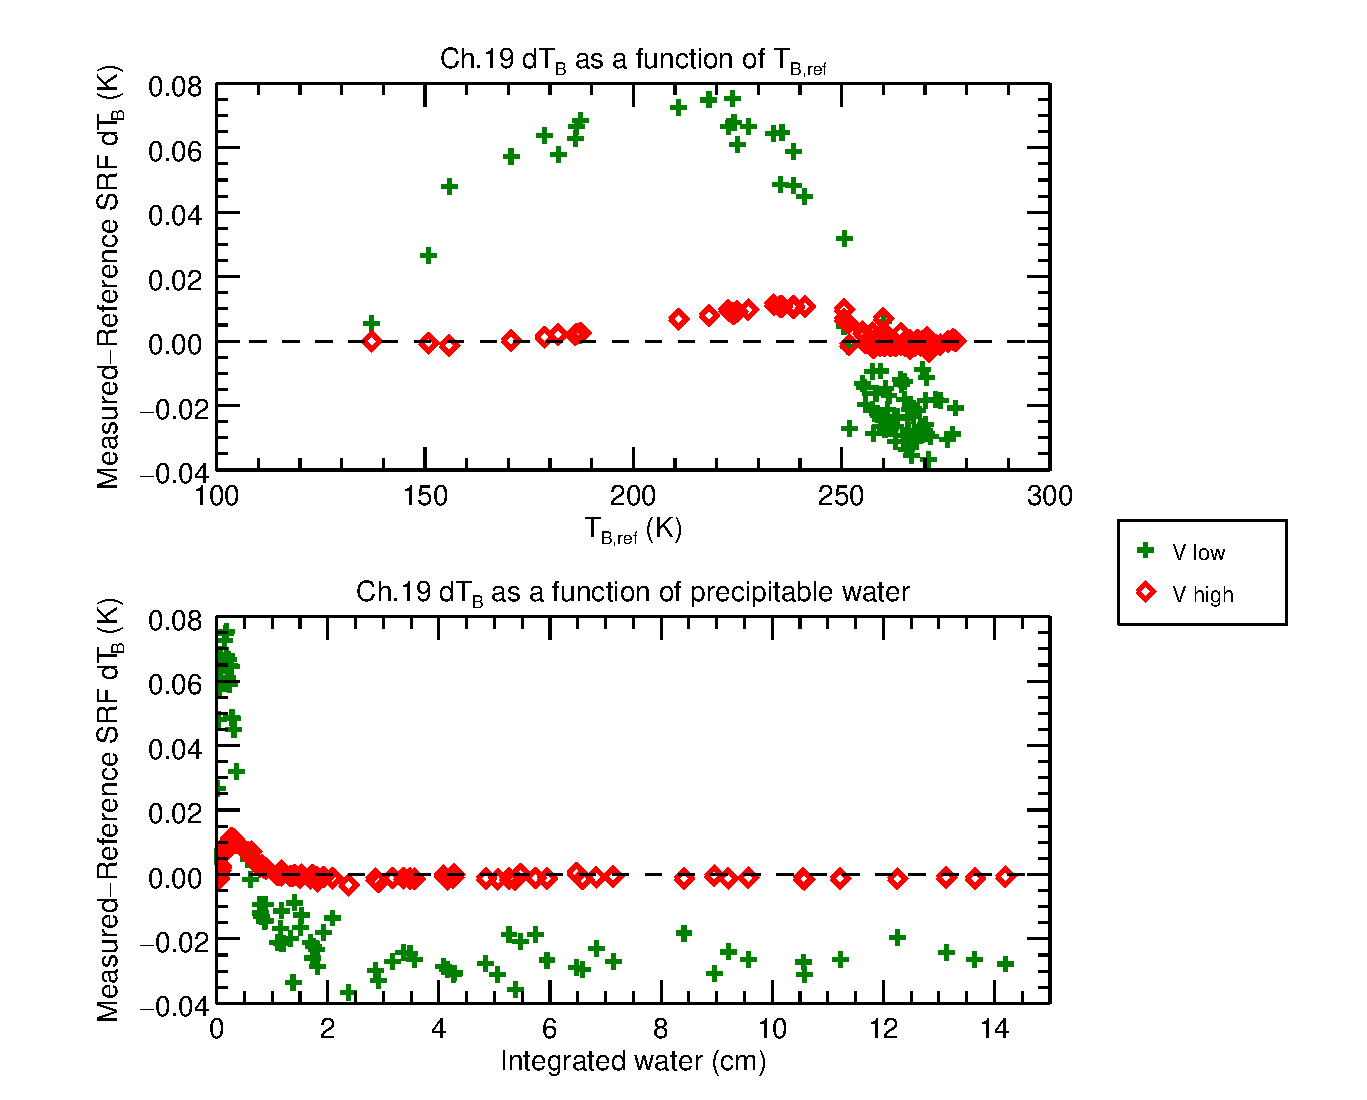
\includegraphics[scale=0.45]{graphics/dtb/Vset/atms_npp.ch19.dTb_T_PW_stats.eps}
  \caption{ATMS channel 19 differences in brightness temperatures as a function of $T_B$ (top) and total preciptable water (bottom) for $V_{LO}$ and $V_{HI}$ compared to nominal bias voltage at nominal temperature (20\textdegree{}C). MonoRTM v5.0 was used with $\epsilon=0.6$ and $r=0.4$ for the ECMWF83 profile set.}
\end{figure}

\subsection{Channel 20}
\begin{figure}[H]
  \label{fig:Vset.ch20_dtb}
  \centering
  \hspace{1.5cm}\includegraphics[scale=0.45]{graphics/dtb/Vset/atms_npp.ch20.dTb_T_PW_stats.eps}
  \caption{ATMS channel 20 differences in brightness temperatures as a function of $T_B$ (top) and total preciptable water (bottom) for $V_{LO}$ and $V_{HI}$ compared to nominal bias voltage at nominal temperature (20\textdegree{}C). MonoRTM v5.0 was used with $\epsilon=0.6$ and $r=0.4$ for the ECMWF83 profile set.}
\end{figure}

\subsection{Channel 21}
\begin{figure}[H]
  \label{fig:Vset.ch21_dtb}
  \centering
  \hspace{1.5cm}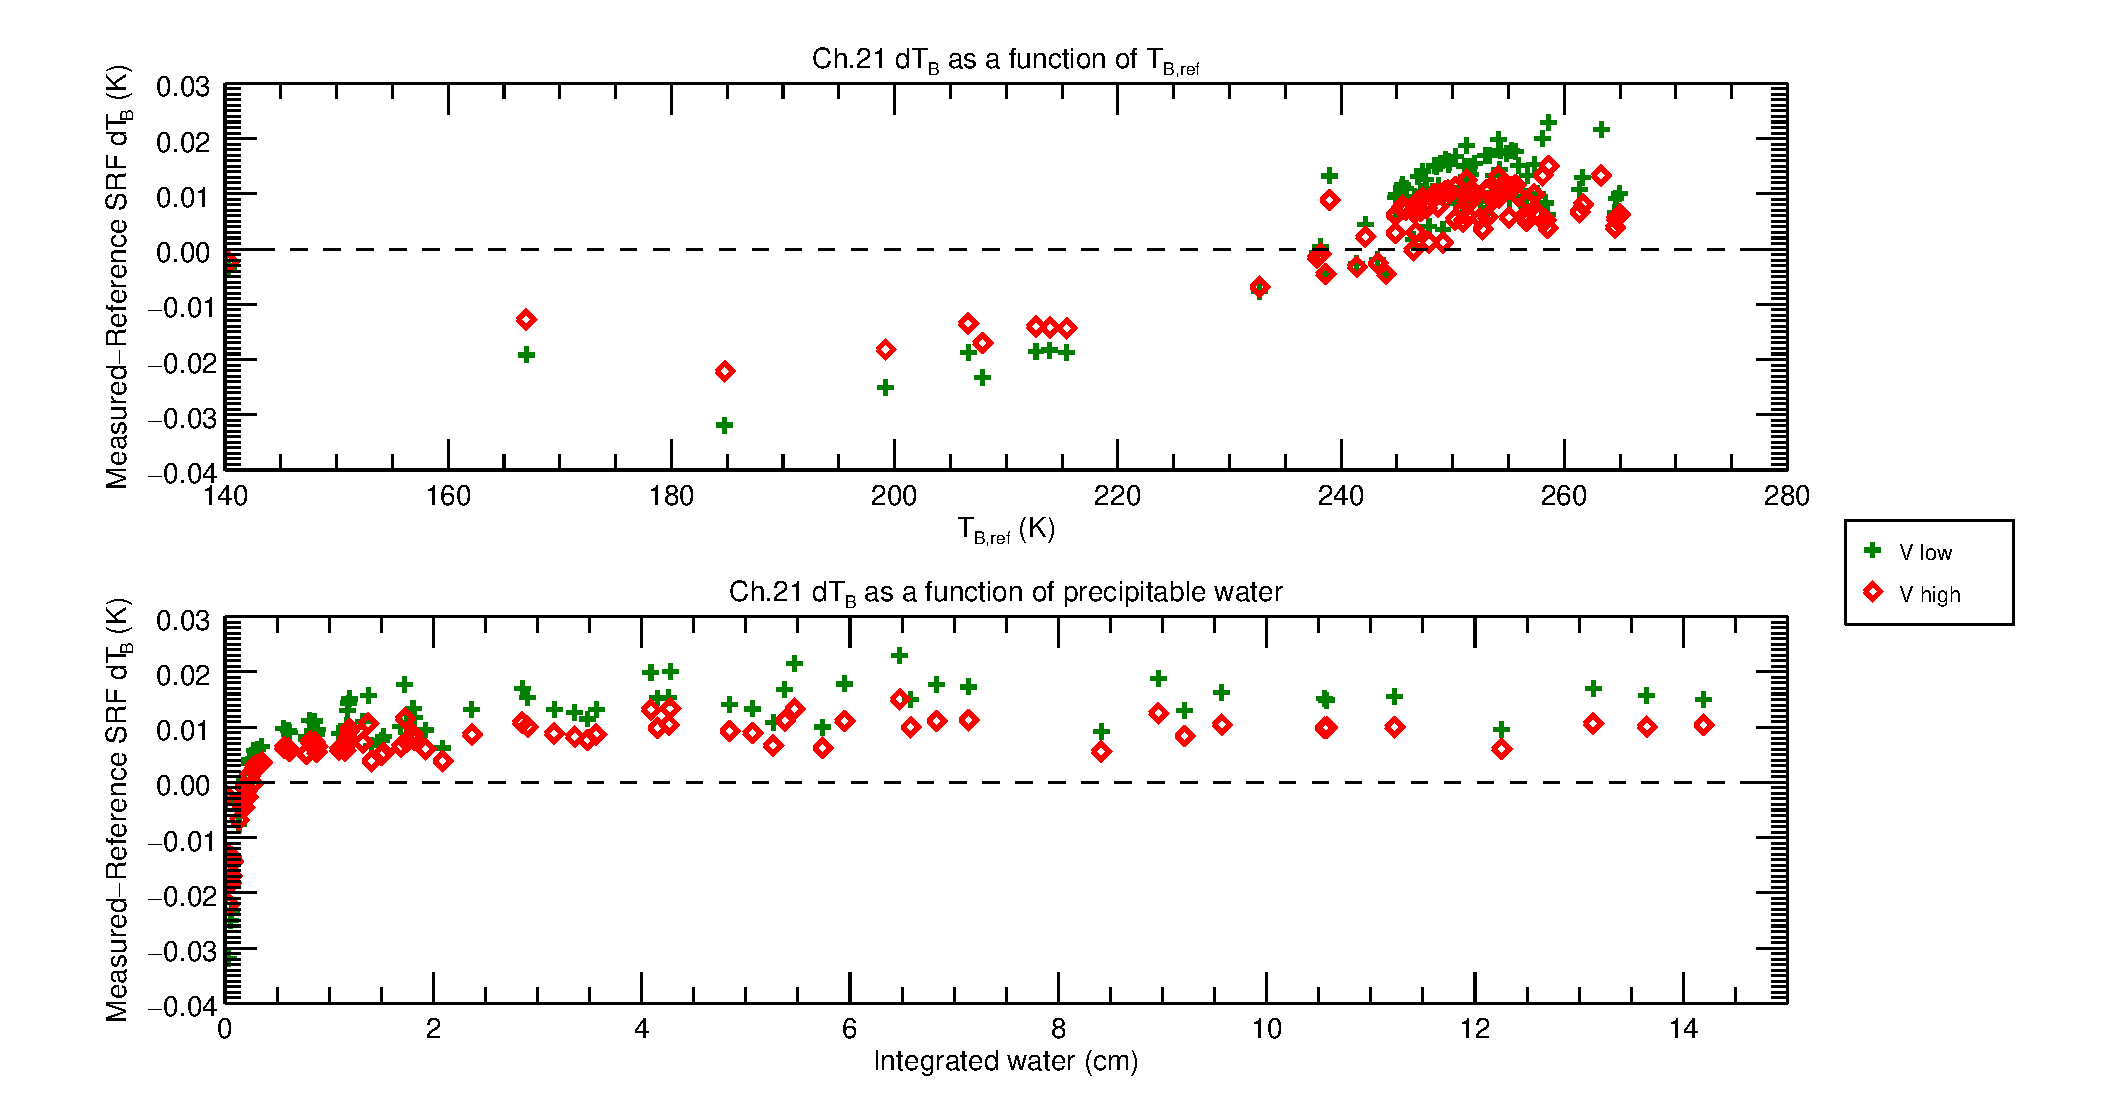
\includegraphics[scale=0.45]{graphics/dtb/Vset/atms_npp.ch21.dTb_T_PW_stats.eps}
  \caption{ATMS channel 21 differences in brightness temperatures as a function of $T_B$ (top) and total preciptable water (bottom) for $V_{LO}$ and $V_{HI}$ compared to nominal bias voltage at nominal temperature (20\textdegree{}C). MonoRTM v5.0 was used with $\epsilon=0.6$ and $r=0.4$ for the ECMWF83 profile set.}
\end{figure}

\subsection{Channel 22}
\begin{figure}[H]
  \label{fig:Vset.ch22_dtb}
  \centering
  \hspace{1.5cm}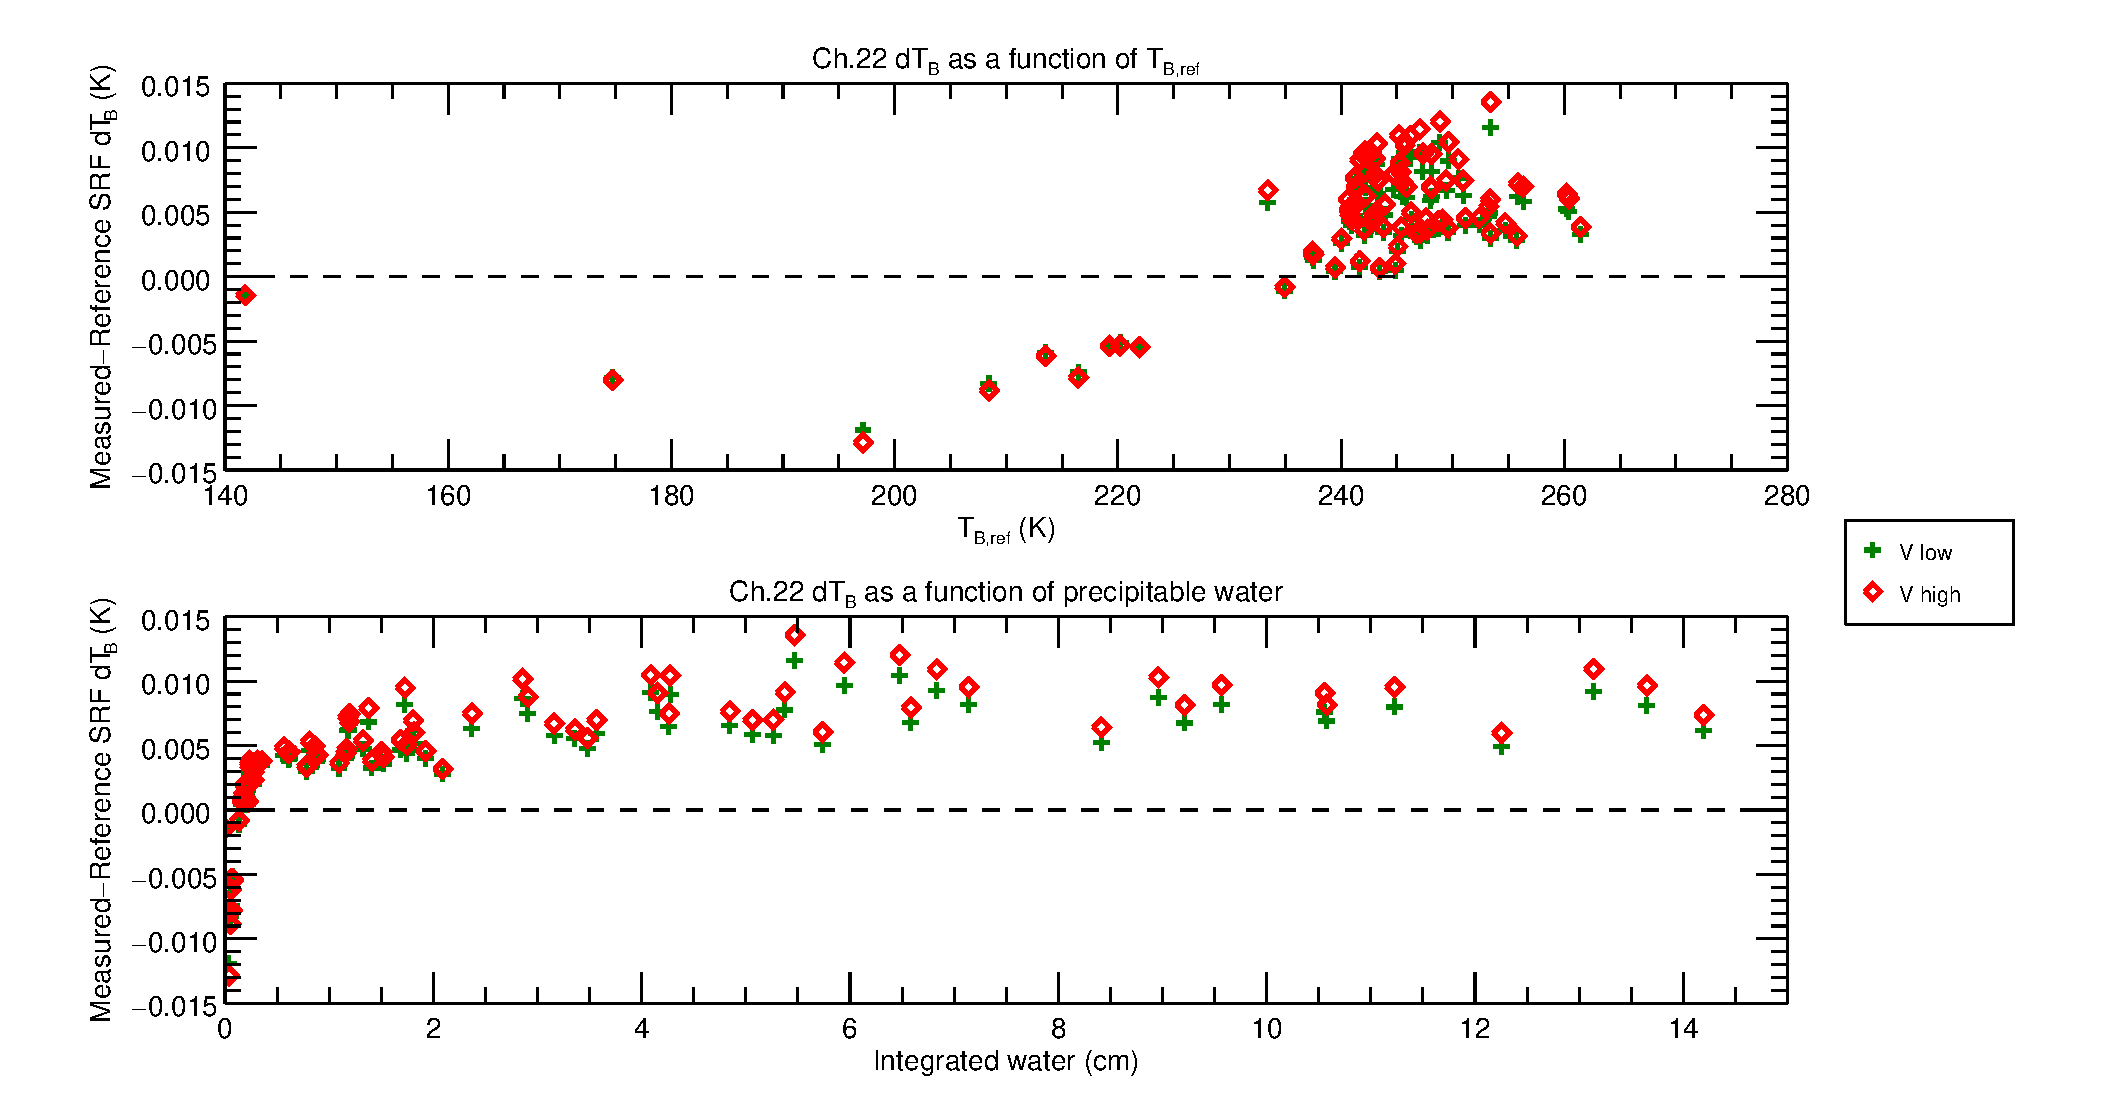
\includegraphics[scale=0.45]{graphics/dtb/Vset/atms_npp.ch22.dTb_T_PW_stats.eps}
  \caption{ATMS channel 22 differences in brightness temperatures as a function of $T_B$ (top) and total preciptable water (bottom) for $V_{LO}$ and $V_{HI}$ compared to nominal bias voltage at nominal temperature (20\textdegree{}C). MonoRTM v5.0 was used with $\epsilon=0.6$ and $r=0.4$ for the ECMWF83 profile set.}
\end{figure}
